% Created by Aly Shmahell
\documentclass[9pt]{extarticle}
\setlength{\parindent}{0.0in}
\usepackage{amsmath}
\usepackage{multicol}
\usepackage{ifluatex}
\ifluatex
\usepackage{pdftexcmds}
\makeatletter
\let\pdfstrcmp\pdf@strcmp
\let\pdffilemoddate\pdf@filemoddate
\makeatother
\fi
\usepackage{svg}
\usepackage{graphicx}
\usepackage{epstopdf}
\epstopdfsetup{outdir=./}
\usepackage[landscape,letterpaper,twoside=false,top=15mm,bottom=15mm,left=10mm,right=10mm]{geometry}
\pagestyle{myheadings}
\markright{}
\usepackage{listings}
\usepackage{color}
\usepackage{pdfpages}
\definecolor{green}{rgb}{0,0.6,0}
\definecolor{blue}{rgb}{0,0,0.6}
\definecolor{orange}{rgb}{0.58,0.2,0}
\definecolor{purple}{RGB}{158,0,160}
\definecolor{eminence}{RGB}{108,48,130}
\definecolor{frenchplum}{RGB}{129,20,83}
\lstset{
	basicstyle=\ttfamily\scriptsize,
	aboveskip={1.5\baselineskip},
	breaklines=true,
	frame=single,
	alsoletter={.,*},
	rulecolor=\color[rgb]{0.75,0.75,0.75},
	showstringspaces=false,
	keywordstyle=\bfseries\color{green},
	commentstyle=\itshape\color{purple},
	identifierstyle=\color{black},
	stringstyle=\color{orange},
	emph=[1]{<,>,vector,string},
	emphstyle=[1]{\color{frenchplum}},
	emph=[2]{NULL,*,\&},
	emphstyle=[2]{\color{red}},
	literate={*}{{\textcolor{blue}{*}}}1,
}
\title{Simplified CKY for NLP}
\author{by: Aly Shmahell}

\begin{document}
	\maketitle
	\begin{multicols*}{3}
		\setlength{\parskip}{0.0in}
		\tableofcontents
		\setlength{\parskip}{0.1in}
		\section{Pseudo-Code}
			\lstinputlisting[language=c++]{pseudo-code.cpp}
		\section{Example}
			\subsection{CFG}
				\lstinputlisting[language=c++]{cfg.txt}
			\subsection{Input}
				\lstinputlisting[language=c++]{input.txt}
			\subsection{Applying SCKY}
				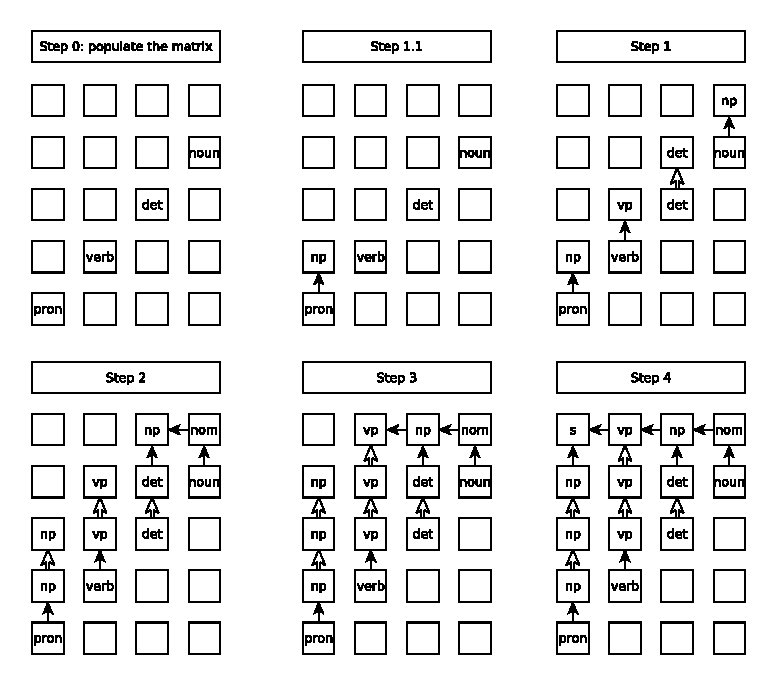
\includegraphics[width=95mm]{example.pdf}	
    \end{multicols*}
\end{document}